\documentclass[11pt,a4paper]{article}
\usepackage[margin=27mm]{geometry}
\usepackage{fontspec,booktabs,array,hyperref,graphicx}
\setmainfont{STIXGeneral}
\setlength{\parindent}{0pt}\setlength{\parskip}{5pt}
\begin{document}
\begin{center}{\Large Complete manuscript comparison}\\[3pt]
Overview v12: symmetric manuscript counts\end{center}
This additive edition restores three whole-topic comparisons and the three affected individual comparisons after exact executable-listing exclusions on both sides. It retains 19 topics and 43 recovered originals among 106 accessible originals; 63 remain pending. Scientific admissions, required proof inputs and the 55 archived originals are unchanged. Expanded E and enlarged Mixes are outside this edition.

The complete written factor is $\sum_i c(S_i)/(c(U)+\sum_i c(A_i))$ within each topic: the whole common paper and every complete application are paid. No theory is free because another topic proves a similar statement. The primary unit is characters without whitespace; each topic retains its published source representation and extraction convention. These are observed manuscript costs, not minimum proof complexities. No pooled factor is formed.
\begin{center}\small\begin{tabular}{lrrrrr}\toprule
Topic & Originals & Sources & Common & Applications & Factor\\\midrule
A & 7 & 213,803 & 49,059 & 87,019 & 1.571 \\
B & 5 & 124,906 & 44,905 & 69,265 & 1.094 \\
C & 5 & 118,433 & 30,437 & 61,248 & 1.292 \\
D & 3 & 47,894 & 15,632 & 29,855 & 1.053 \\
E & 3 & 71,375 & 19,790 & 19,513 & 1.816 \\
F & 2 & 69,825 & 15,876 & 27,398 & 1.614 \\
G & 2 & 73,199 & 30,928 & 85,207 & 0.630 \\
Affine & 1 & 32,767 & 19,070 & 22,638 & 0.786 \\
Representation & 1 & 25,348 & 11,288 & 13,688 & 1.015 \\
Chamber & 2 & 34,177 & 15,199 & 21,254 & 0.938 \\
Matching & 1 & 37,951 & 16,732 & 17,168 & 1.119 \\
ChiralEnumeration & 1 & 27,594 & 8,831 & 23,171 & 0.862 \\
Operations & 3 & 200,630 & 58,215 & 100,379 & 1.265 \\
Gluing & 1 & 27,081 & 28,416 & 11,565 & 0.677 \\
RankContraction & 1 & 15,530 & 6,937 & 10,555 & 0.888 \\
LocallyProjective & 2 & 26,490 & 25,498 & 11,966 & 0.707 \\
MathieuCensus & 1 & 13,736 & 5,516 & 35,862 & 0.332 \\
RankAugmentation & 1 & 33,604 & 13,904 & 14,096 & 1.200 \\
Mixes & 1 & 57,753 & 12,615 & 31,077 & 1.322 \\
\bottomrule\end{tabular}\end{center}
The exact 19-row \href{topics.csv}{topic CSV} retains historical costs and fractions alongside current values. Chamber, ChiralEnumeration and Operations now use the matched listing boundary. The other 16 topic records are unchanged. A factor below one remains visible.
\newpage
\section*{Individual comparisons: first 22 originals}
After acquiring the \emph{whole} common theory and all required proof, program and data premises for that topic, the conditional factor is $c(S_i)/c(A_i)$. Every complete local application or companion bundle is charged. Optional validation is not relabeled as a premise.
\begin{center}\small\begin{tabular}{llrrr}\toprule
Original & Topic & Source & Application & Factor\\\midrule
L032 & A & 16,558 & 8,212 & 2.016 \\
L034 & A & 21,433 & 5,784 & 3.706 \\
F016 & A & 43,983 & 15,419 & 2.853 \\
F013 & A & 25,562 & 6,224 & 4.107 \\
L035 & A & 51,019 & 14,498 & 3.519 \\
N009 & A & 36,824 & 28,114 & 1.310 \\
L128 & A & 18,424 & 8,768 & 2.101 \\
N001 & B & 14,519 & 7,371 & 1.970 \\
N003 & B & 17,780 & 9,155 & 1.942 \\
N008 & B & 18,009 & 11,132 & 1.618 \\
L030 & B & 22,704 & 12,286 & 1.848 \\
L040 & B & 51,894 & 29,321 & 1.770 \\
L088 & C & 13,166 & 11,311 & 1.164 \\
N013 & C & 27,361 & 15,815 & 1.730 \\
L108 & C & 12,849 & 10,075 & 1.275 \\
F014 & C & 20,577 & 6,962 & 2.956 \\
L068 & C & 44,480 & 17,085 & 2.603 \\
L066 & D & 20,916 & 10,989 & 1.903 \\
L074 & D & 20,661 & 13,367 & 1.546 \\
L104 & D & 6,317 & 5,499 & 1.149 \\
L083 & E & 20,885 & 3,002 & 6.957 \\
L079 & E & 20,908 & 1,855 & 11.271 \\\bottomrule\end{tabular}\end{center}
Only L008, L028 and N006 change. Their source listings were previously included while replacement code was excluded. Current source costs remove the exact reviewed blocks; application costs remain unchanged. The other 40 conditional fractions retain their earlier values, including N016, N005 and N007. All 43 rows, exact fractions and acquisition conditions are in \href{applications.csv}{applications.csv}.

Programs implementing proofs keep that logical role even when their listing text is excluded symmetrically from a manuscript comparison. The complete program and mandatory-data inventories remain separately bound. There is no software-inclusive or optional-validation-inclusive scalar: historical source software costs are unknown.
\newpage
\section*{Individual comparisons: remaining 21 originals}
\begin{center}\small\begin{tabular}{llrrr}\toprule
Original & Topic & Source & Application & Factor\\\midrule
L021 & E & 29,582 & 14,656 & 2.018 \\
L014 & F & 25,574 & 11,504 & 2.223 \\
L007 & F & 44,251 & 15,894 & 2.784 \\
L009 & G & 49,891 & 23,544 & 2.119 \\
L092 & G & 23,308 & 61,663 & 0.378 \\
L012 & Affine & 32,767 & 22,638 & 1.447 \\
F010 & Representation & 25,348 & 13,688 & 1.852 \\
L008 & Chamber & 20,159 & 7,571 & 2.663 \\
N016 & Chamber & 14,018 & 13,683 & 1.024 \\
F015 & Matching & 37,951 & 17,168 & 2.211 \\
L028 & ChiralEnumeration & 27,594 & 23,171 & 1.191 \\
N005 & Operations & 122,002 & 49,595 & 2.460 \\
N006 & Operations & 55,740 & 38,479 & 1.449 \\
N007 & Operations & 22,888 & 12,305 & 1.860 \\
L010 & Gluing & 27,081 & 11,565 & 2.342 \\
L037 & RankContraction & 15,530 & 10,555 & 1.471 \\
L084 & LocallyProjective & 2,071 & 4,857 & 0.426 \\
L095 & LocallyProjective & 24,419 & 7,109 & 3.435 \\
L073 & MathieuCensus & 13,736 & 35,862 & 0.383 \\
L020 & RankAugmentation & 33,604 & 14,096 & 2.384 \\
F005 & Mixes & 57,753 & 31,077 & 1.858 \\\bottomrule\end{tabular}\end{center}
\textbf{Exact exclusions.} L008: three Magma functions, section 5, physical pages 8--10. L028: the ChiralPolytopes, OrderedSubsetsGroups and DiagramPlus implementations, section 4.2, physical pages 9--12. N006: the McL search pseudocode in the Theorem 5.3 proof, physical page 20. Seven blocks are removed in twelve page chunks; surrounding proof, comments outside those blocks, Lemma 4.5, mathematical algorithm prose, presentations and tables remain. No whole section is discarded.

\textbf{Limits and sensitivity.} The listing audit covers the measured text and supplied replacement TeX; it is not a claim about unseen software or unextracted graphics. Operations retains its proposed text proxies for source diagrams, with a separate text-only sensitivity in the matched numerical packet. That sensitivity is not substituted for the primary coordinate; graphic complexity remains unknown. The matched packet preserves all 30 coordinates per topic, plus ten text-only Operations coordinates. Unknown external proofs, source software, historical costs and complete formalization costs are null, not zero. Partial Lean checks are not full source formalization.

The prior v10 and v11 costs, factors and held statuses remain historical records. This edition supplies current graphs without changing scientific admissions or adding source, question or formalization credit.
\newpage
\section*{Whole topics}
Grey bars show complete original manuscript text under each row's declared convention. Replacement bars stack whole common theory and all applications. The axis starts at zero. These are lengths; ratios are shown in the tables.
\begin{center}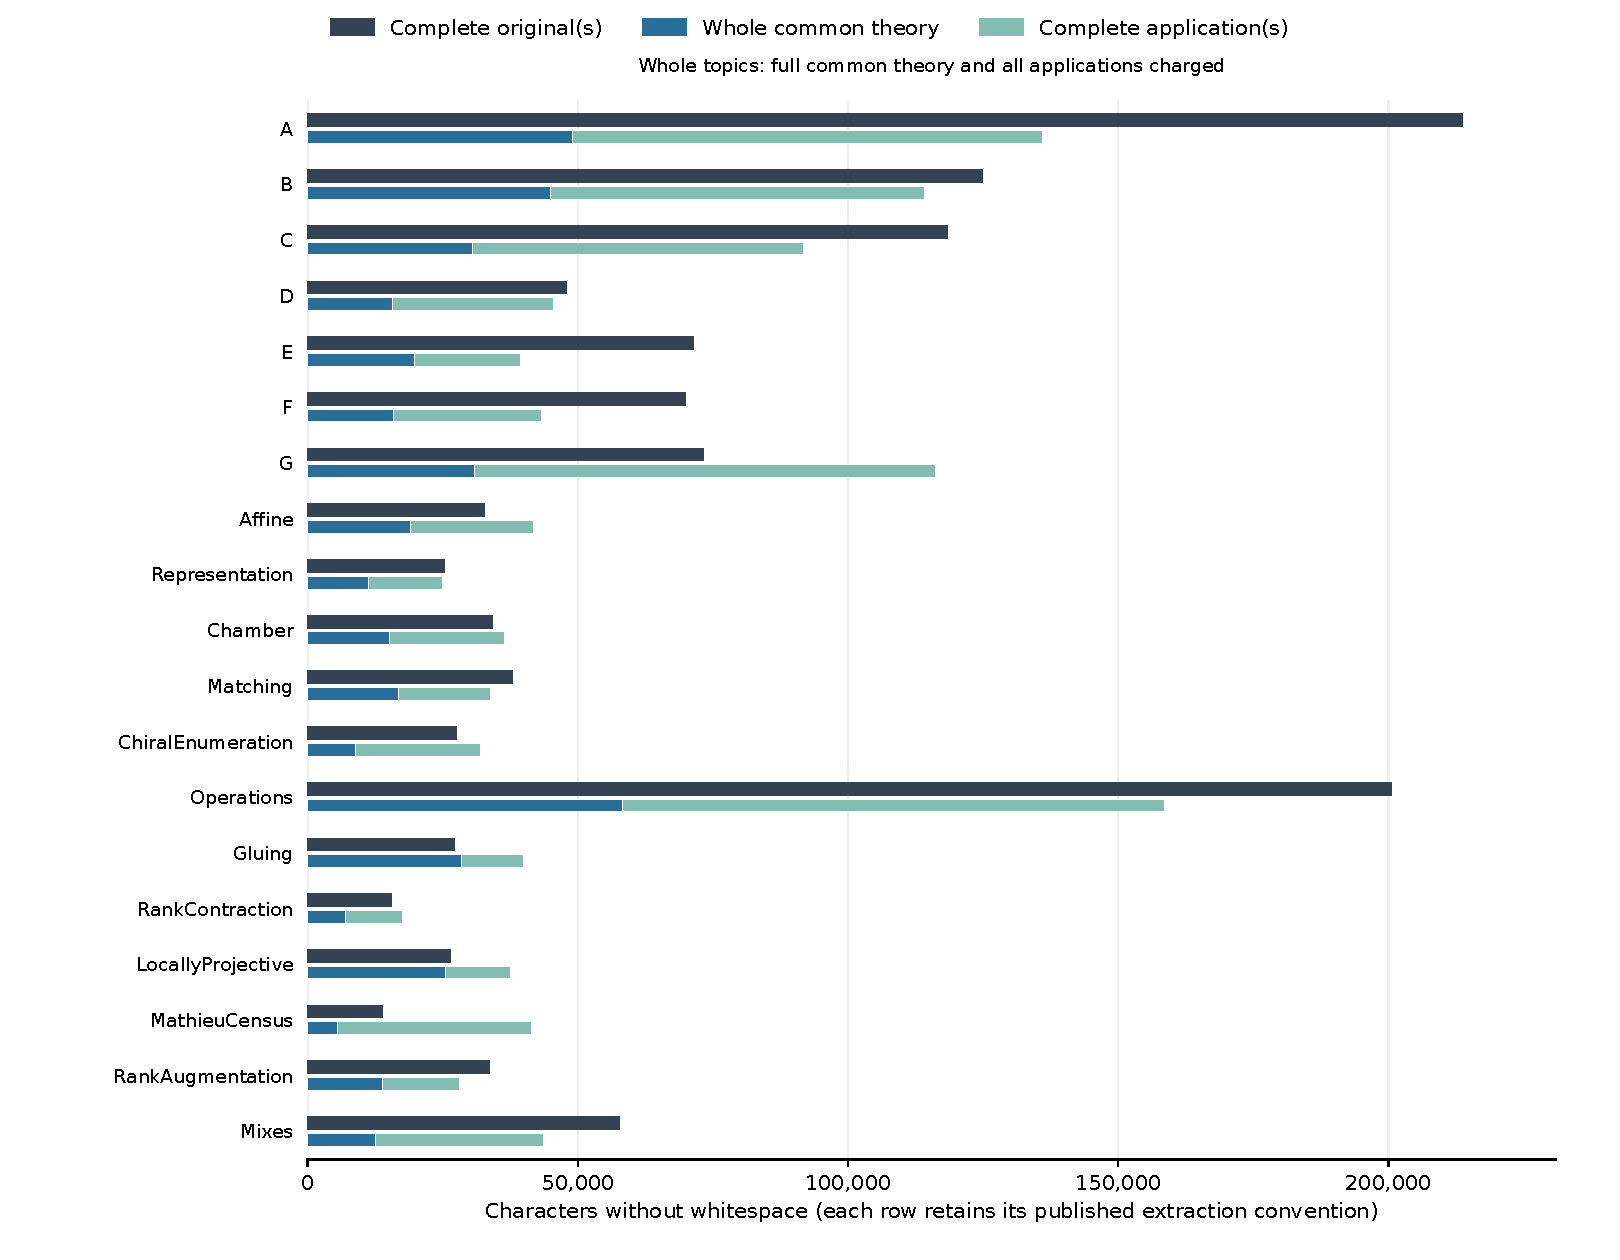
\includegraphics[width=\linewidth]{whole_topics.pdf}\end{center}
The entire common contribution remains visible, including theory needed only by some applications. The 57 actual bars correspond to all 19 topics.
\newpage
\section*{Conditional lengths: first 22 originals}
The common theory and required premises are acquired in advance. Grey and teal bars compare complete source and local application text; they do not remove that prerequisite cost from the whole-topic table.
\begin{center}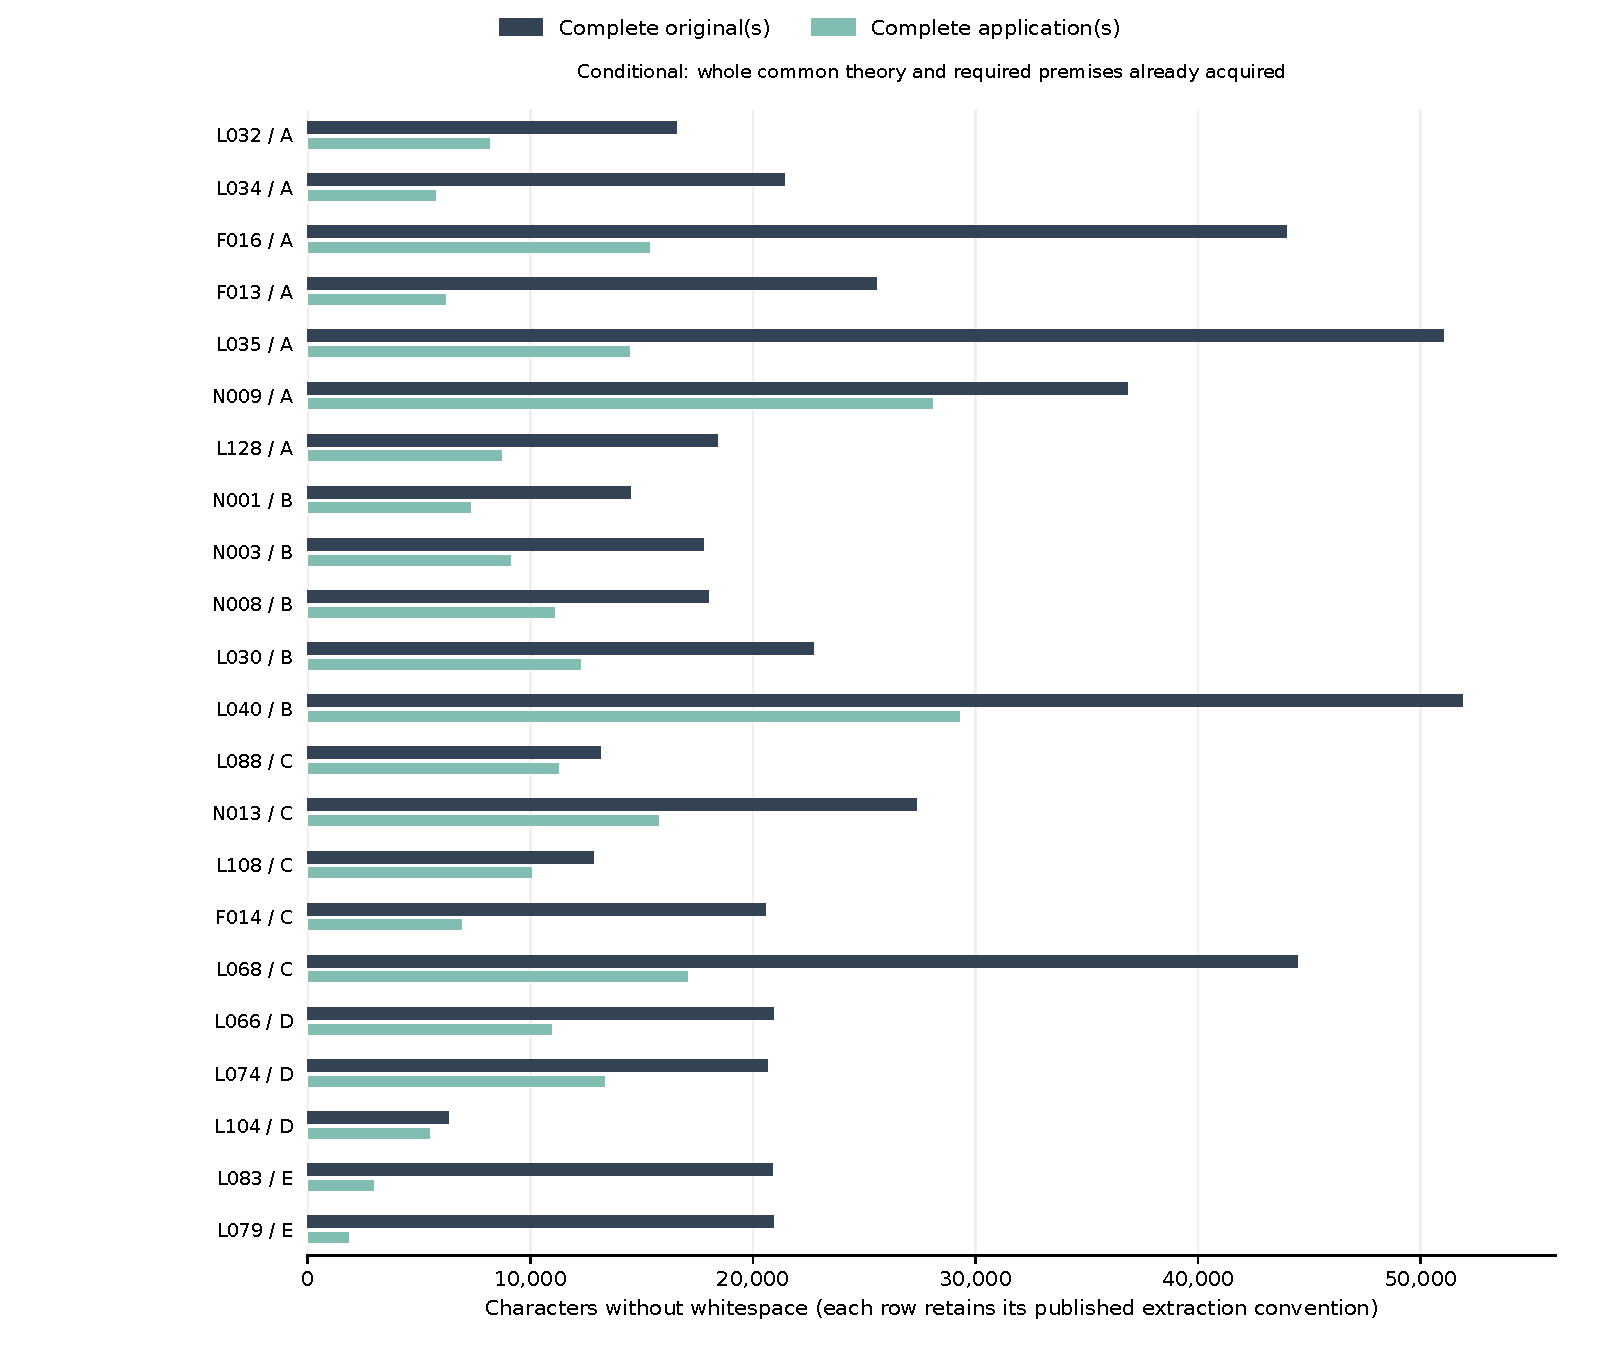
\includegraphics[width=\linewidth]{conditional_1.pdf}\end{center}
\newpage
\section*{Conditional lengths: remaining 21 originals}
The acquisition condition is identical for every row. There is no cross-topic discount and no inferred sawtooth or node-count factor.
\begin{center}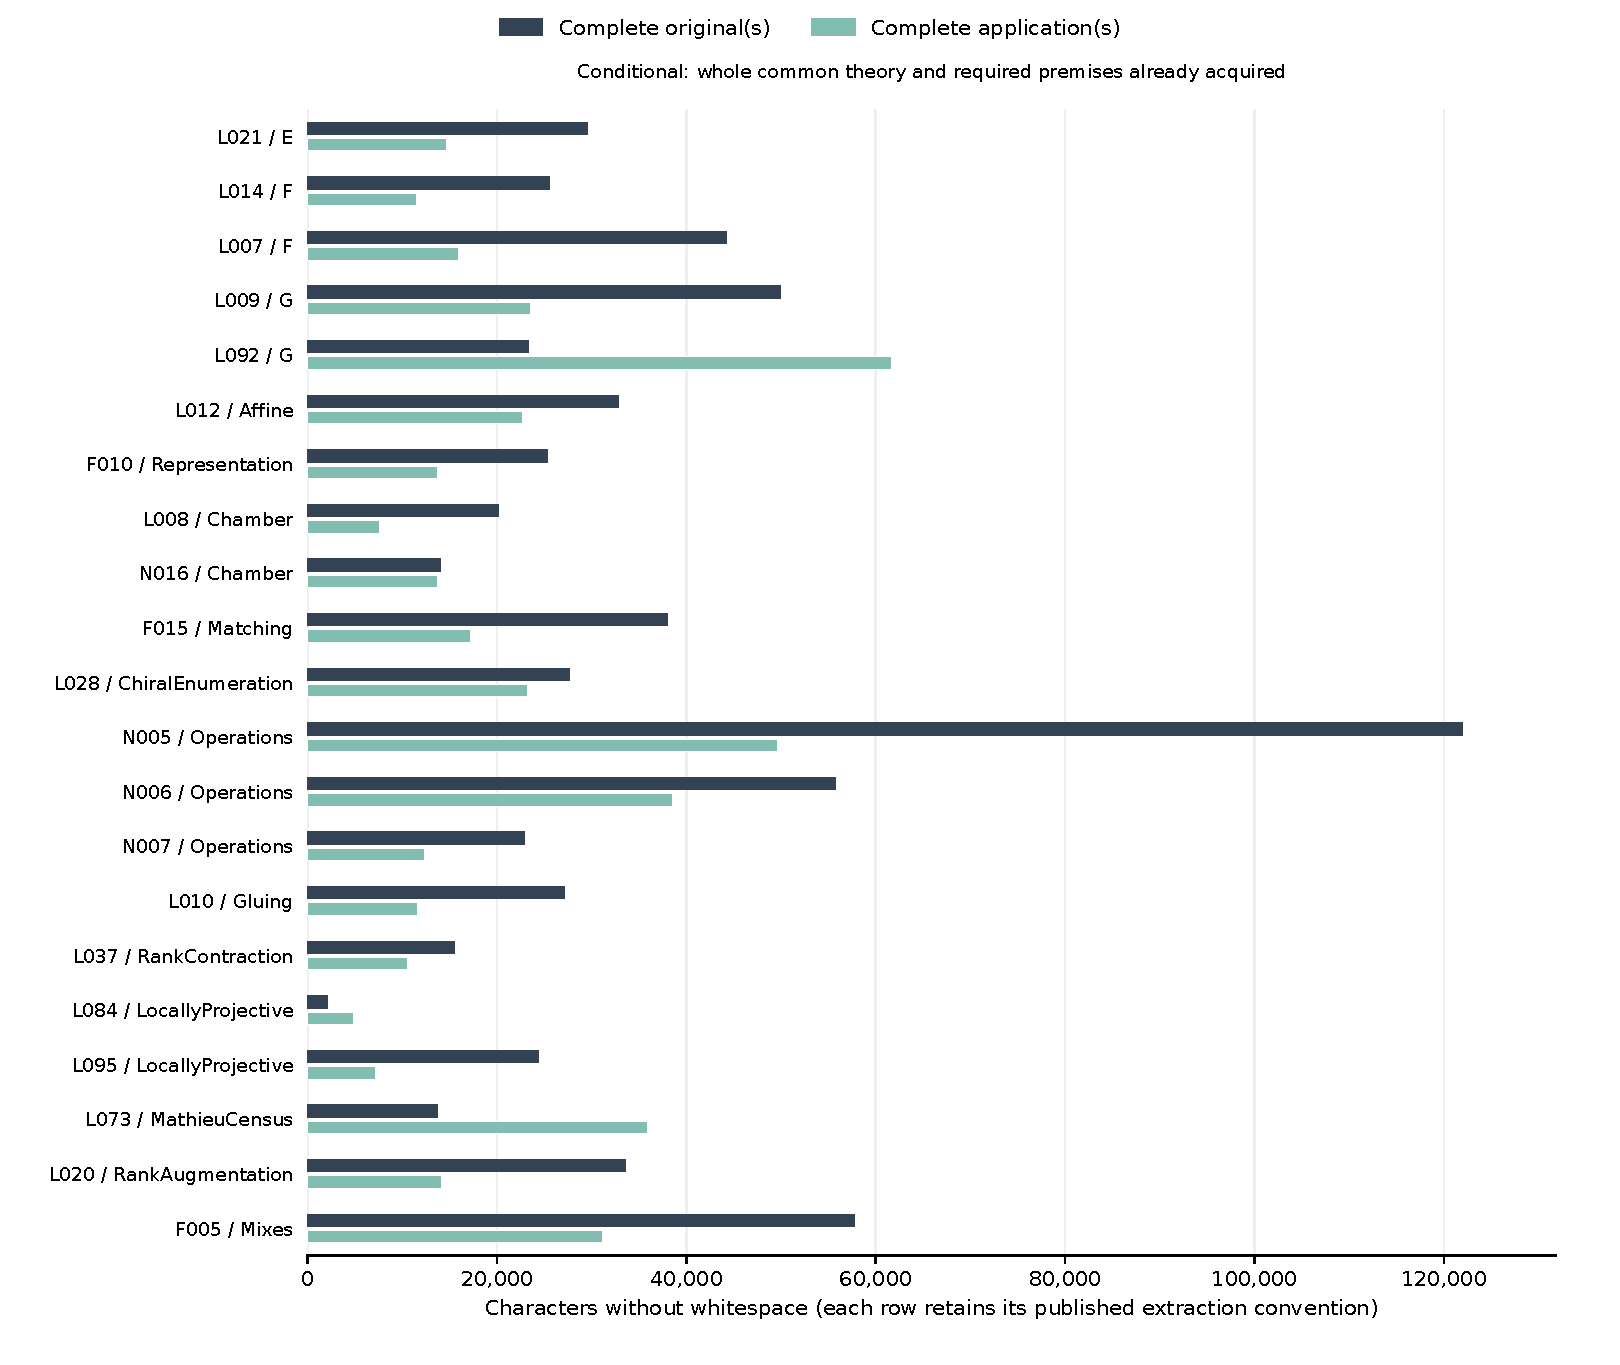
\includegraphics[width=\linewidth]{conditional_2.pdf}\end{center}
\end{document}
